\section*{3. Stellar classification}

Figure 2. presents the relative line strengths, for different elements and molecules, for different types
of stars. This can be used to classify stars into different stellar types, depending on which elements
cause absorption features in the stellar spectrum.\\
\\

\noindent\makebox[\textwidth]{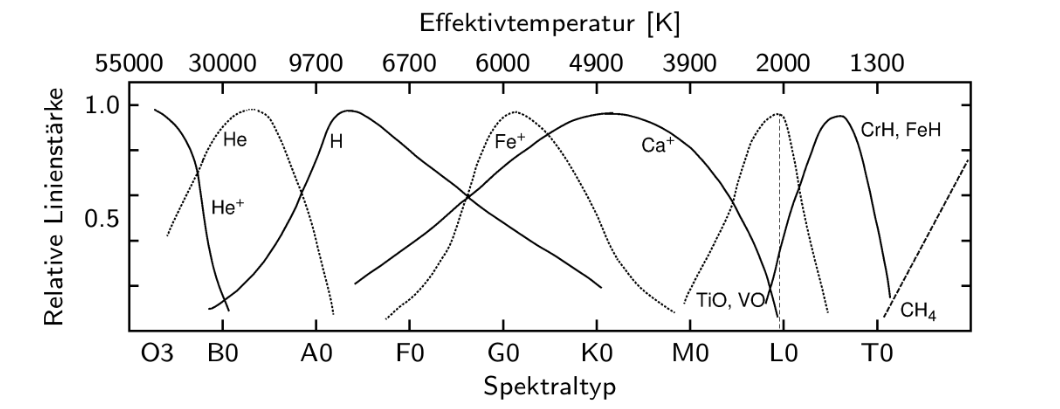
\includegraphics[scale=0.05]{spectrum.png}}\\

Figure 2: Diagram shows the relative absorption line strength in dependence of the stellar spectral 
type.\\
\\
a) To get an idea of which energies different elements absorb, have a look at the Frauenhofer lines and
write down the elements and their line energies that could help you classify the spectra shown in part
(b) of this question.\\
\\
b) Figure 3 shows the spectra of 5 different stars. Use the information from part (a) to estimate the
spectral type of each star and state the reasons for you choosing this type. It is sufficient to mention
the letter connected with the spectral class (O, B, A, F, G, K, M), while sub-classes do not need to be
estimated.\\
\\

\noindent\makebox[\textwidth]{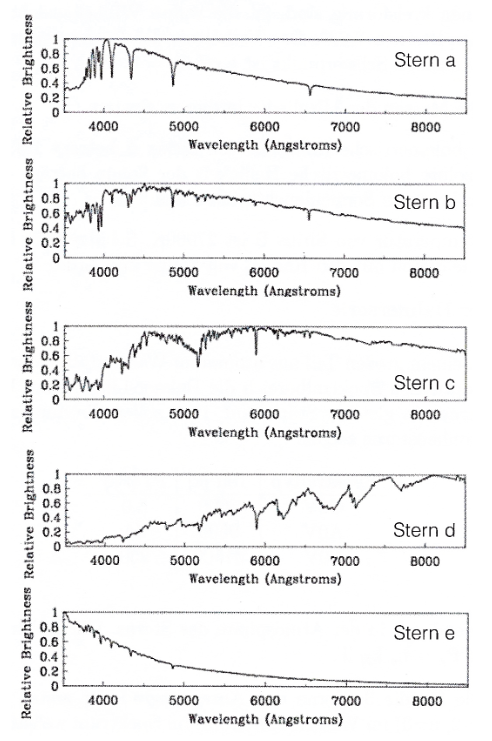
\includegraphics[scale=0.05]{spectras.png}}\\

Figure 3: Stellar spectra in the optical wavelength regime for 5 different stars.\\
\\
